% CS615A Aspects of System Administration
% Author: Jan Schaumann <jschauma@netmeister.org>
% $Id: slides.tex,v 1.11 2006/02/07 03:55:59 jschauma Exp $

\special{! TeXDict begin /landplus90{true}store end }

\documentclass[xga]{xdvislides}
\usepackage[landscape]{geometry}
\usepackage{graphics}
\usepackage{graphicx}
\usepackage{colordvi}

\begin{document}
\setfontphv

%%% Headers and footers
\lhead{\slidetitle}                               % default:\lhead{\slidetitle}
\chead{CS615 - Aspects of System Administration}% default:\chead{\relax}
\rhead{Slide \thepage}                       % default:\rhead{\sectiontitle}
\lfoot{\Gray{Lecture 03: Software Installation Concepts}}% default:\lfoot{\slideauthor}
\cfoot{\relax}                               % default:\cfoot{\relax}
\rfoot{\Gray{\today}}

\vspace*{\fill}
\begin{center}
	\Hugesize
		CS615 - Aspects of System Administration\\ [1em]
		Software Installation Concepts \\ [1em]
	\hspace*{5mm}\blueline\\ [1em]
	\Normalsize
		Department of Computer Science\\
		Stevens Institute of Technology\\
		Jan Schaumann\\
		\verb+jschauma@stevens.edu+ \\
		\verb+http://www.cs.stevens.edu/~jschauma/615/+
\end{center}
\vspace*{\fill}

\subsection{Last week...}
\begin{center}
	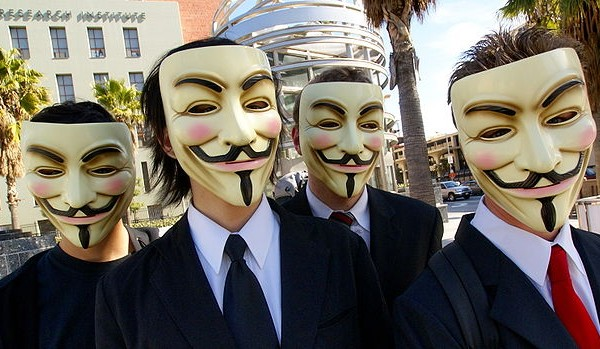
\includegraphics[scale=0.6]{pics/anonymous.eps}
\\
{\tt http://pastebin.com/8G4jLha8}
\\
{\tt https://www.cs.columbia.edu/\~{}smb/blog/2012-02/2012-02-05.html}
\end{center}

\subsection{Types of Software}
\subsection{Firmware}
\begin{center}
	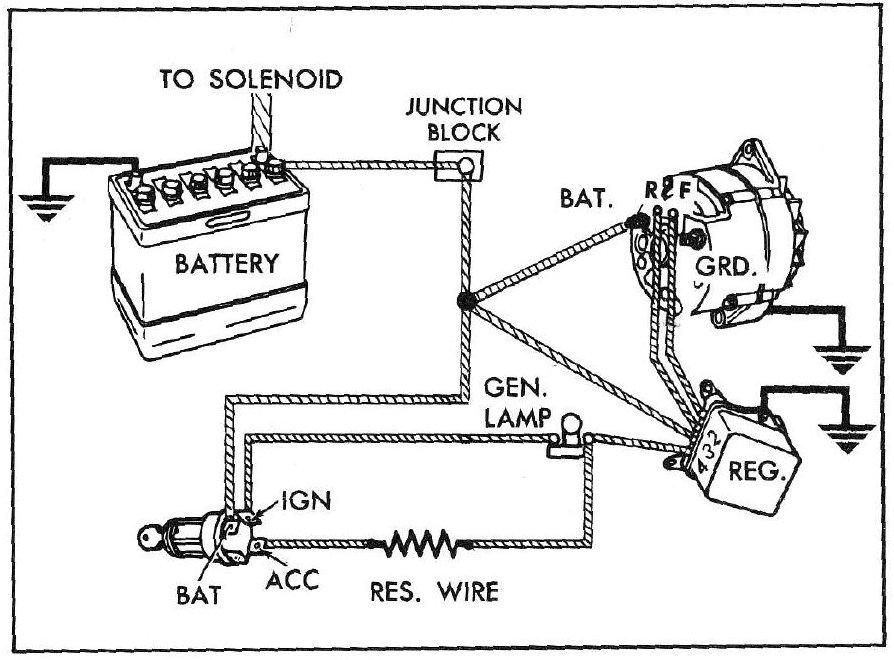
\includegraphics[scale=0.6,angle=-90]{pics/ignition-firmware.eps}
\end{center}

\subsection{Firmware}
\begin{center}
	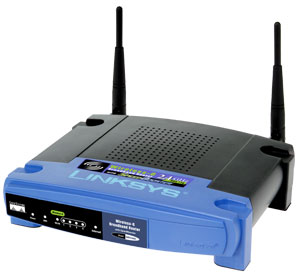
\includegraphics[scale=0.6,angle=-90]{pics/linksys.eps}
	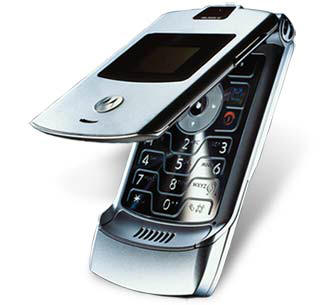
\includegraphics[scale=0.6,angle=-90]{pics/cell-phone.eps}
	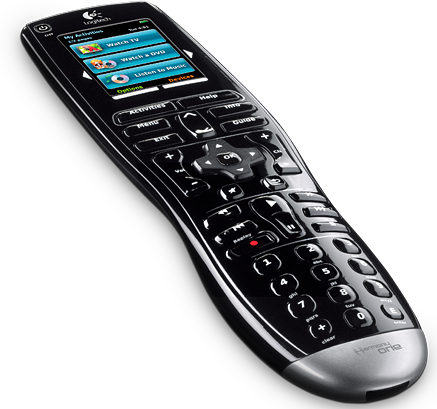
\includegraphics[scale=0.4,angle=-90]{pics/remote.eps}
\end{center}

\subsection{Firmware}
\begin{center}
	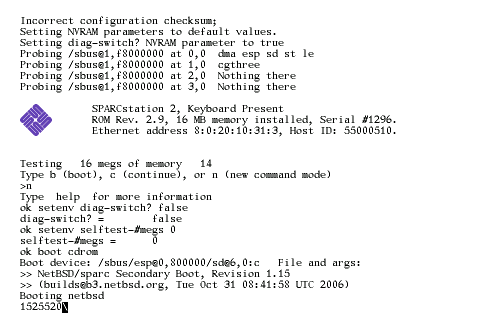
\includegraphics[scale=0.9,angle=-90]{pics/sun-firmware.eps}
\end{center}

\subsection{Firmware}
\begin{center}
	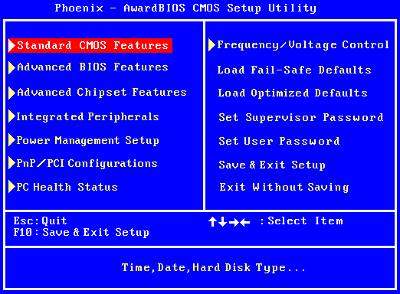
\includegraphics[scale=0.9,angle=-90]{pics/BIOS.eps}
\end{center}

\subsection{...}
\begin{center}
	
\includegraphics[scale=0.9]{pics/kfc1.eps}
\end{center}

\subsection{Kernel}
\begin{center}
	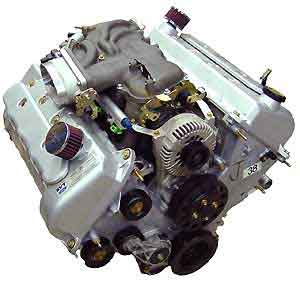
\includegraphics[scale=0.95,angle=-90]{pics/engine-kernel.eps}
\end{center}

\subsection{Kernel}
\begin{center}
	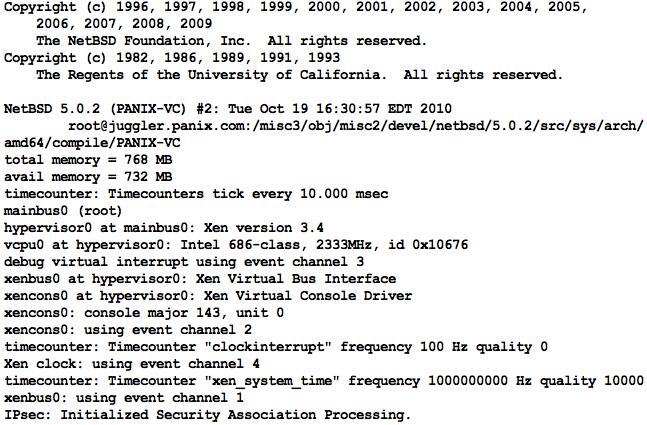
\includegraphics[scale=0.7,angle=-90]{pics/kernel-dmesg.eps}
\end{center}

\subsection{OS}
\begin{center}
	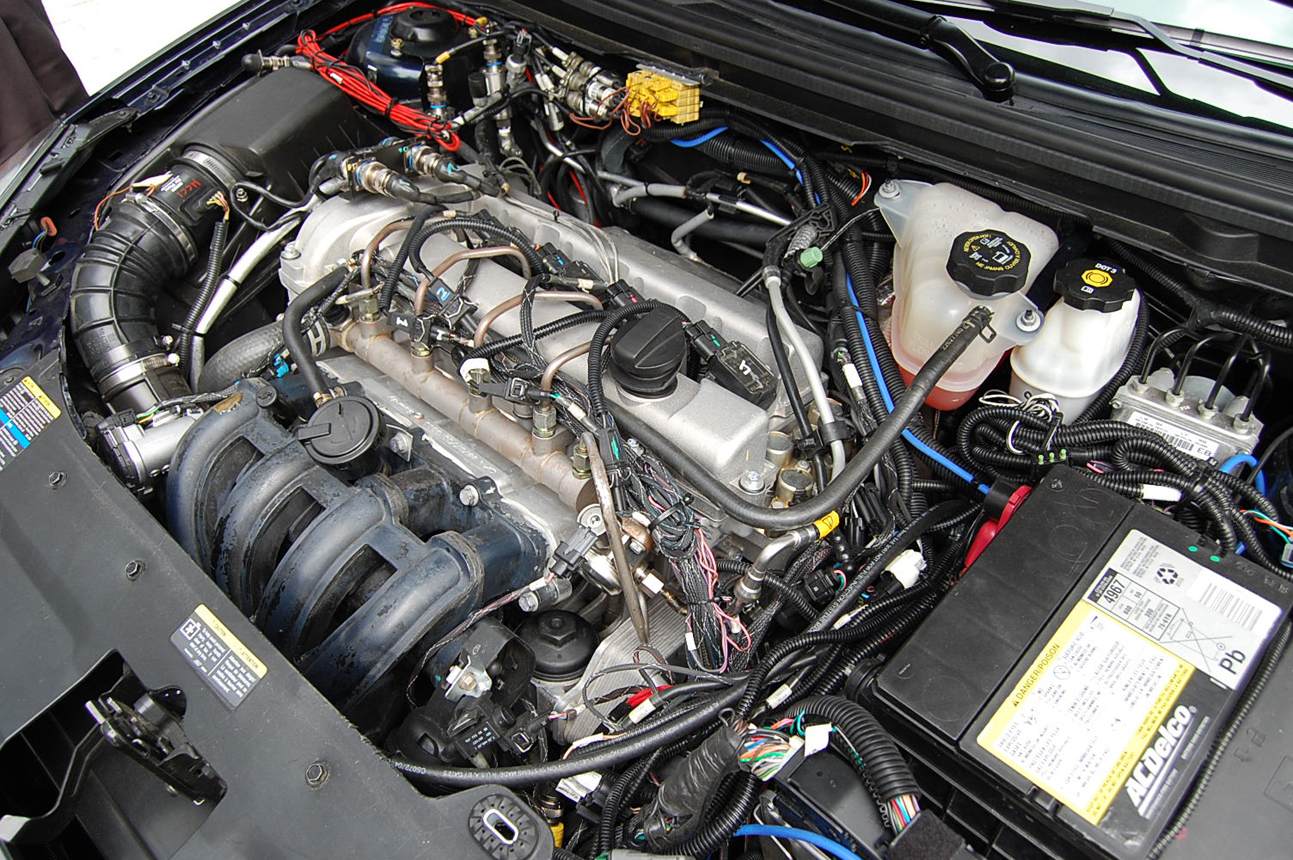
\includegraphics[scale=0.7,angle=-90]{pics/engine-os.eps}
\end{center}

\subsection{OS}
\begin{center}
	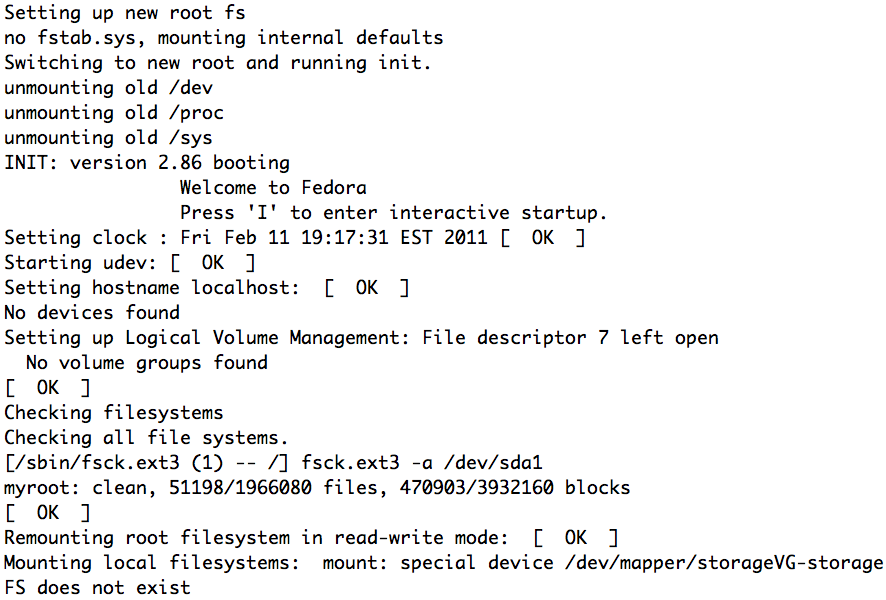
\includegraphics[scale=0.6,angle=-90]{pics/os-screenshot.eps}
\end{center}

\subsection{System Software}
\begin{center}
	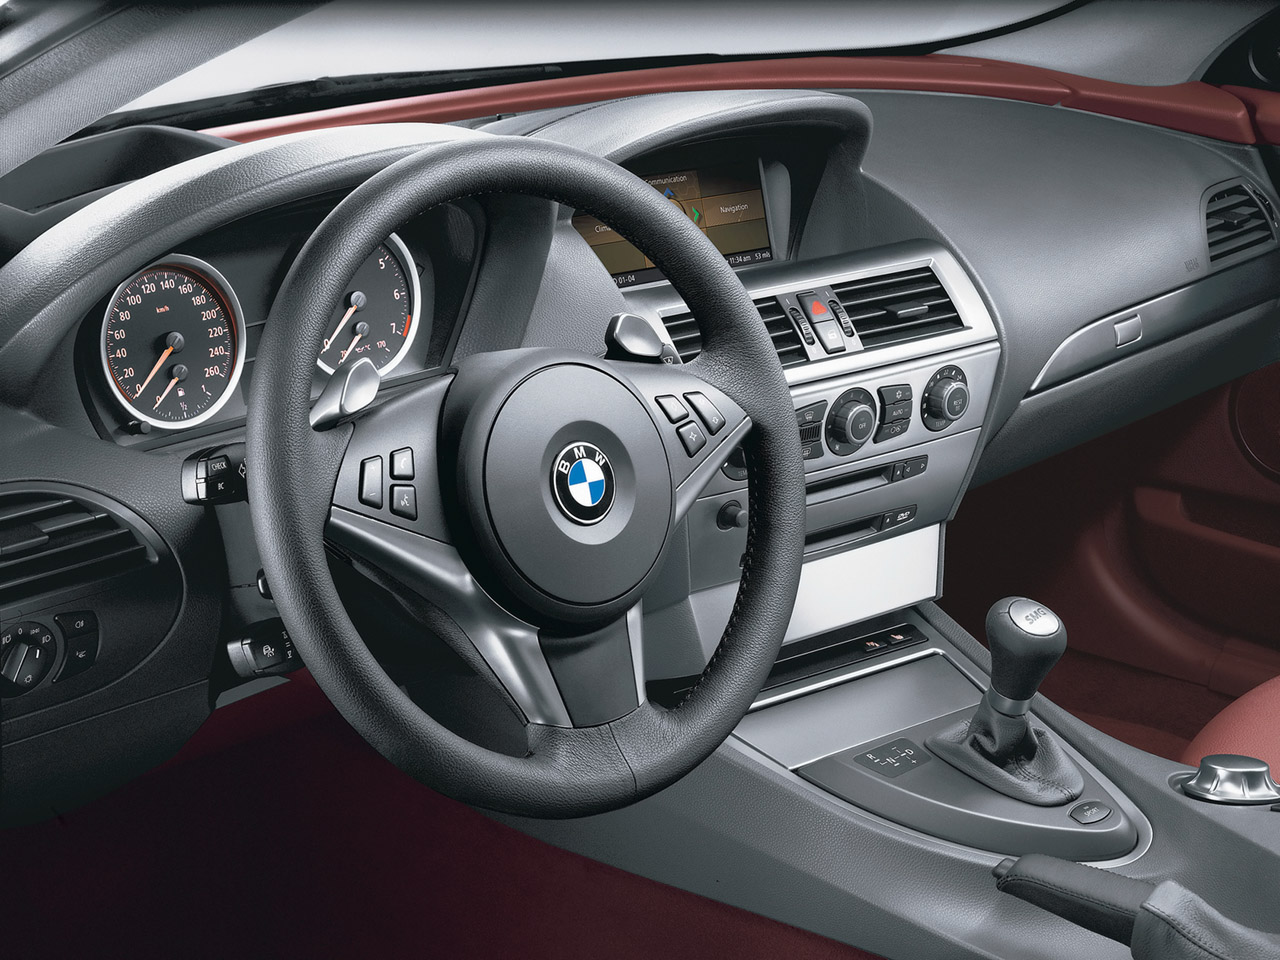
\includegraphics[scale=0.6,angle=-90]{pics/dashboard-system-software.eps}
\end{center}

\subsection{System Software}
\begin{center}
	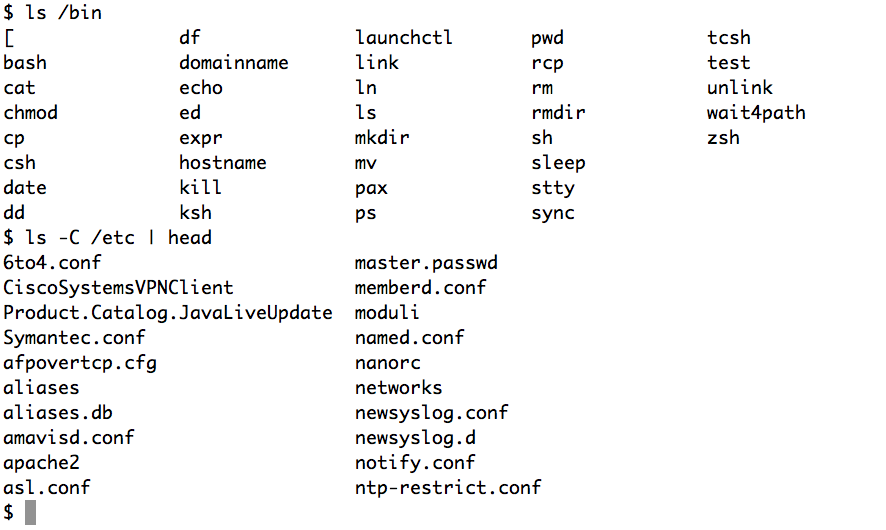
\includegraphics[scale=0.7,angle=-90]{pics/system-software.eps}
\end{center}

\subsection{Applications}
\begin{center}
	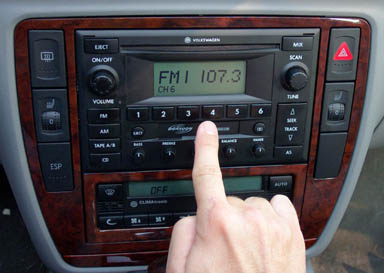
\includegraphics[scale=0.9,angle=-90]{pics/car_radio-applications.eps}
\end{center}

\subsection{Applications}
\begin{center}
	
\includegraphics[scale=0.3,angle=-90]{pics/python.eps}
	
\includegraphics[scale=0.3,angle=-90]{pics/logo_oracle.eps}
	\includegraphics[scale=0.8,angle=-90]{pics/apache.eps} \\
	
\includegraphics[scale=0.3,angle=-90]{pics/mysql.eps}
	
\includegraphics[scale=0.3,angle=-90]{pics/php-logo.eps}
\end{center}

\subsection{Typical Boot Sequence}
\begin{itemize}
	\item {\bf P}ower-{\bf o}n {\bf S}elf-{\bf T}est
	\item primary boot loader (BIOS, UEFI, Open Firmware / OpenBoot)
	\item transfer of execution to {\bf M}aster {\bf B}oot {\bf R}ecord or perform netbooting
	\item Second-stage boot loader (GRUB, LILO, etc.)
	\item load kernel
	\item kernel transfers control to {\tt init(8)}
\end{itemize}

\subsection{Topics covered}
\begin{itemize}
	\item OS installation
\end{itemize}

\subsection{Topics covered}
\begin{itemize}
	\item OS installation
	\item file system hierarchy
\end{itemize}

\subsection{Topics covered}
\begin{itemize}
	\item OS installation
	\item file system hierarchy
	\item system software vs. third party software
\end{itemize}

\subsection{Topics covered}
\begin{itemize}
	\item OS installation
	\item file system hierarchy
	\item system software vs. third party software
	\item binary installation
\end{itemize}

\subsection{Topics covered}
\begin{itemize}
	\item OS installation
	\item file system hierarchy
	\item system software vs. third party software
	\item binary installation
	\item installation from source
\end{itemize}


\subsection{Topics covered}
\begin{itemize}
	\item OS installation
	\item file system hierarchy
	\item system software vs. third party software
	\item binary installation
	\item installation from source
	\item different package managers
\end{itemize}

\subsection{Topics covered}
\begin{itemize}
	\item OS installation
	\item file system hierarchy
	\item system software vs. third party software
	\item binary installation
	\item installation from source
	\item different package managers
	\item security patches
\end{itemize}

\subsection{No more: ``It's mine!''}
\begin{center}
	
\includegraphics[scale=0.8]{pics/gollum.eps}
\end{center}

\subsection{Kids like to share!}
\begin{center}
	\includegraphics[scale=0.7,angle=-90]{pics/sharing.eps}
\end{center}

\subsection{Eat your own dogfood!}
\begin{center}
	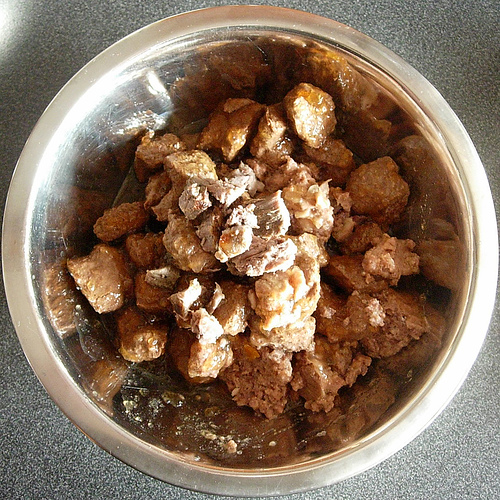
\includegraphics[scale=0.7]{pics/dogfood.eps}
\end{center}



\subsection{OS Installation}
\begin{center}
	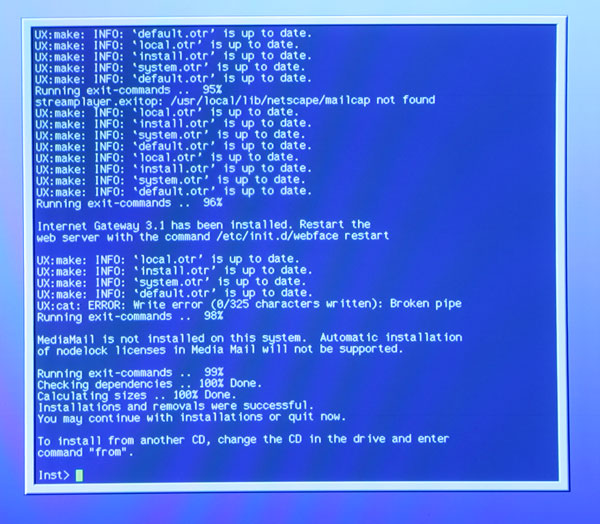
\includegraphics[scale=0.7,angle=-90]{pics/irix-install.eps}
\end{center}

\subsection{OS Installation}
\begin{center}
	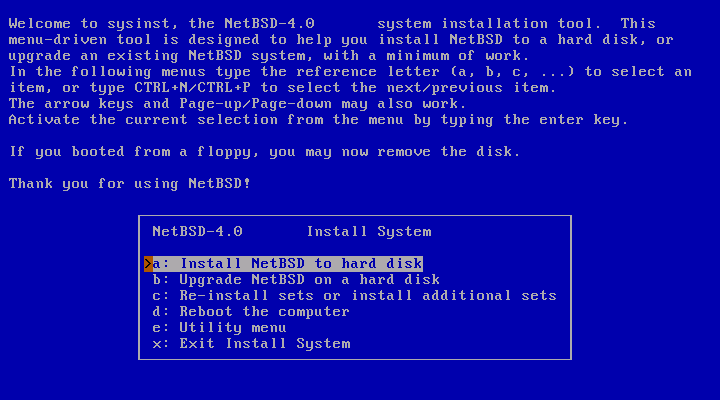
\includegraphics[scale=0.8,angle=-90]{pics/netbsd-install.eps}
\end{center}

\subsection{OS Installation}
\begin{center}
	\includegraphics[scale=0.8,angle=-90]{pics/solaris-install.eps}
\end{center}


\subsection{OS Installation}
Before installing, consider
\begin{itemize}
	\item purpose of machine
\end{itemize}

\subsection{OS Installation}
Before installing, consider
\begin{itemize}
	\item purpose of machine
		\begin{itemize}
			\item choice of hardware
		\end{itemize}
\end{itemize}

\subsection{OS Installation}
Before installing, consider
\begin{itemize}
	\item purpose of machine
		\begin{itemize}
			\item choice of hardware
			\item disk partitioning scheme
		\end{itemize}
\end{itemize}

\subsection{OS Installation}
Before installing, consider
\begin{itemize}
	\item purpose of machine
		\begin{itemize}
			\item choice of hardware
			\item disk partitioning scheme
			\item choice of filesystem
		\end{itemize}
\end{itemize}

\subsection{OS Installation}
Before installing, consider
\begin{itemize}
	\item purpose of machine
		\begin{itemize}
			\item choice of hardware
			\item disk partitioning scheme
			\item choice of filesystem
			\item which software to install
		\end{itemize}
\end{itemize}

\subsection{OS Installation}
Before installing, consider
\begin{itemize}
	\item purpose of machine
		\begin{itemize}
			\item choice of hardware
			\item disk partitioning scheme
			\item choice of filesystem
			\item which software to install
		\end{itemize}
	\item installation media
\end{itemize}

\subsection{OS Installation}
\begin{center}
	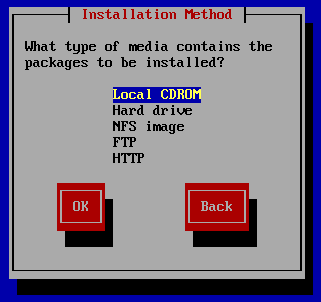
\includegraphics[scale=1.0,angle=-90]{pics/install-method.eps}
\end{center}

\subsection{OS Installation}
Before installing, consider
\begin{itemize}
	\item purpose of machine
		\begin{itemize}
			\item choice of hardware
			\item disk partitioning scheme
			\item choice of filesystem
			\item which software to install
		\end{itemize}
	\item installation media
		\begin{itemize}
			\item network installation
		\end{itemize}
\end{itemize}

\subsection{OS Installation}
Before installing, consider
\begin{itemize}
	\item purpose of machine
		\begin{itemize}
			\item choice of hardware
			\item disk partitioning scheme
			\item choice of filesystem
			\item which software to install
		\end{itemize}
	\item installation media
		\begin{itemize}
			\item network installation
			\item installation CD-ROMs
		\end{itemize}
\end{itemize}

\subsection{OS Installation}
Before installing, consider
\begin{itemize}
	\item purpose of machine
		\begin{itemize}
			\item choice of hardware
			\item disk partitioning scheme
			\item choice of filesystem
			\item which software to install
		\end{itemize}
	\item installation media
		\begin{itemize}
			\item network installation
			\item installation CD-ROMs
			\item customized boot media
		\end{itemize}
\end{itemize}

\subsection{OS Installation}
Before installing, consider
\begin{itemize}
	\item installation process
\end{itemize}

\subsection{OS Installation}
Before installing, consider
\begin{itemize}
	\item installation process
		\begin{itemize}
			\item base installation
		\end{itemize}
\end{itemize}

\subsection{OS Installation}
Before installing, consider
\begin{itemize}
	\item installation process
		\begin{itemize}
			\item base installation
			\item installation of add-ons and third-party applications
		\end{itemize}
\end{itemize}

\subsection{OS Installation}
Before installing, consider
\begin{itemize}
	\item installation process
		\begin{itemize}
			\item base installation
			\item installation of add-ons and third-party applications
			\item security implications
		\end{itemize}
\end{itemize}

\subsection{OS Installation}
Before installing, consider
\begin{itemize}
	\item installation process
		\begin{itemize}
			\item base installation
			\item installation of add-ons and third-party applications
			\item security implications
			\item able to be easily repeated
		\end{itemize}
\end{itemize}

\subsection{OS Installation}
\begin{center}
	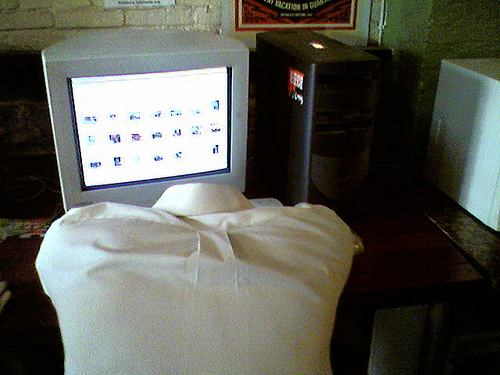
\includegraphics[scale=1.0]{pics/headless.eps}
\end{center}

\subsection{OS Installation}
\vspace*{\fill}
\begin{center}
	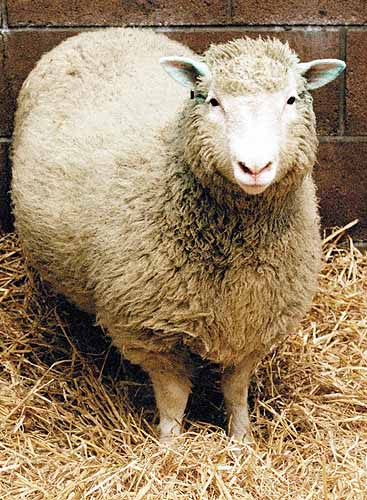
\includegraphics[scale=0.6]{pics/dolly.eps}
\end{center}
\vspace*{\fill}

\subsection{OS Installation}
\vspace*{\fill}
\begin{center}
	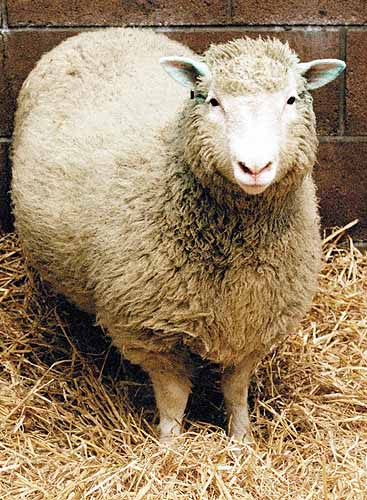
\includegraphics[scale=0.6]{pics/dolly.eps}
	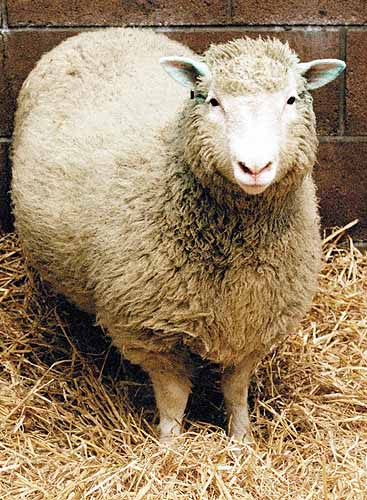
\includegraphics[scale=0.6]{pics/dolly.eps}
\end{center}
\vspace*{\fill}

\subsection{OS Installation}
\vspace*{\fill}
\begin{center}
	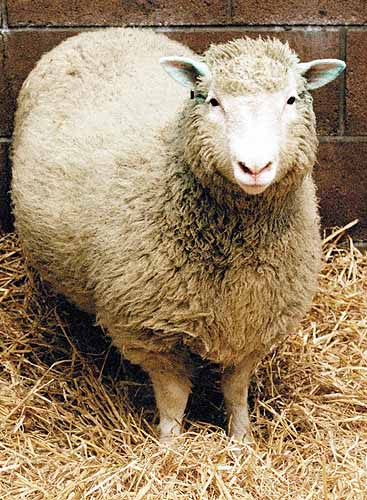
\includegraphics[scale=0.3]{pics/dolly.eps}
	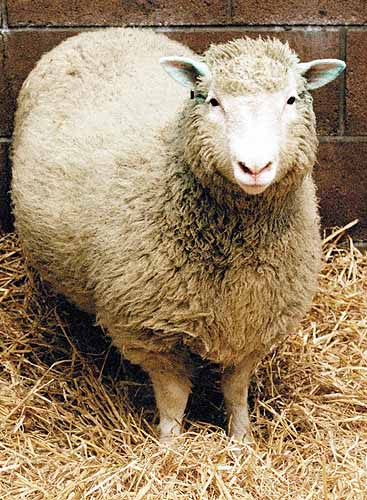
\includegraphics[scale=0.3]{pics/dolly.eps}
	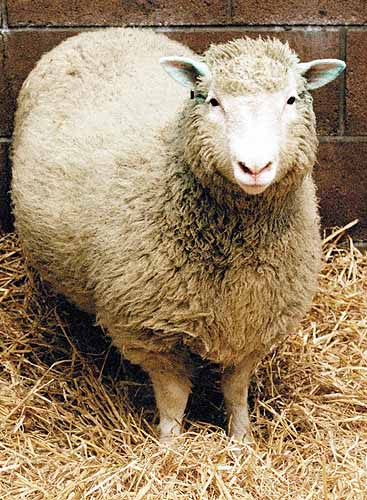
\includegraphics[scale=0.3]{pics/dolly.eps}
	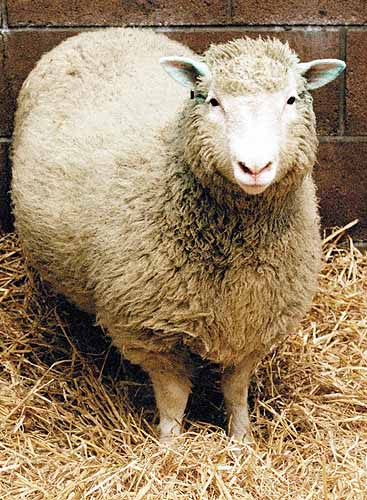
\includegraphics[scale=0.3]{pics/dolly.eps}
	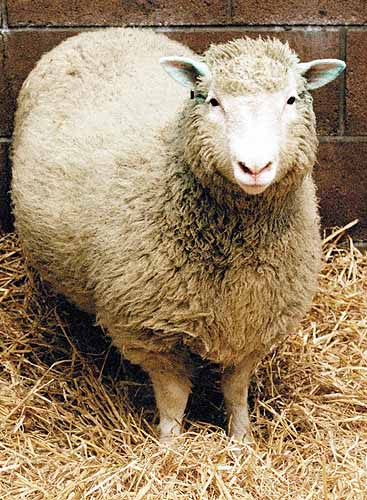
\includegraphics[scale=0.3]{pics/dolly.eps} \\
	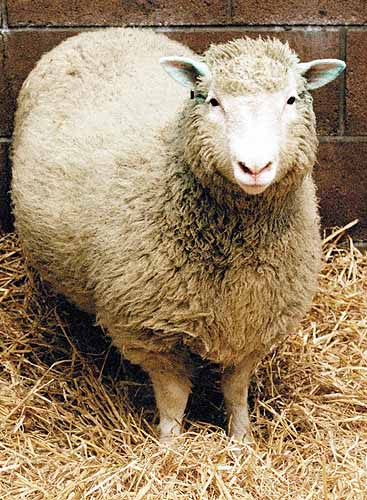
\includegraphics[scale=0.3]{pics/dolly.eps}
	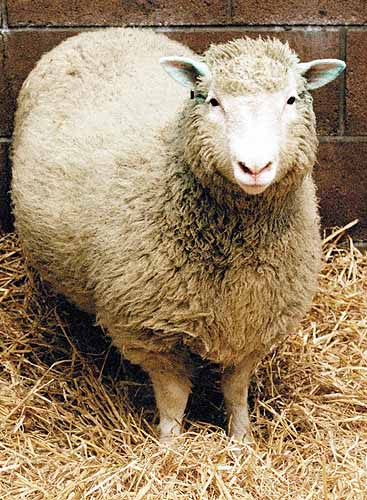
\includegraphics[scale=0.3]{pics/dolly.eps}
	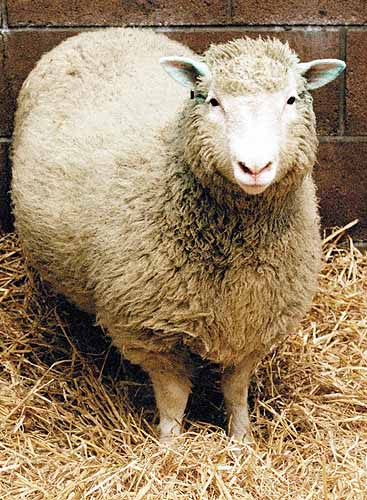
\includegraphics[scale=0.3]{pics/dolly.eps}
	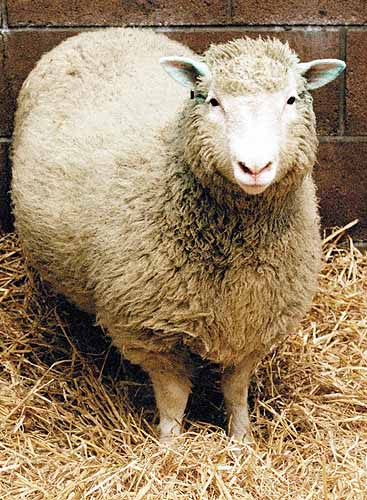
\includegraphics[scale=0.3]{pics/dolly.eps}
	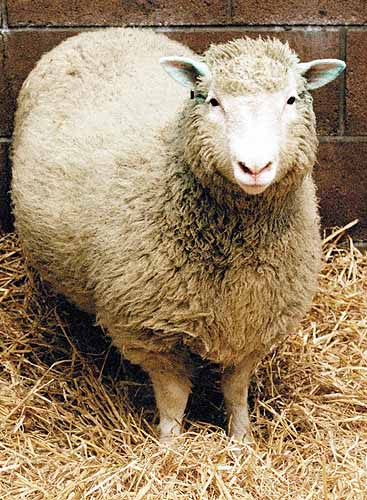
\includegraphics[scale=0.3]{pics/dolly.eps}
\end{center}
\vspace*{\fill}

\subsection{OS Installation}
Before installing, consider
\begin{itemize}
	\item installation process
		\begin{itemize}
			\item base installation
			\item installation of add-ons and third-party applications
			\item security implications
			\item able to be easily repeated
		\end{itemize}
	\item post-installation
\end{itemize}

\subsection{OS Installation}
Before installing, consider
\begin{itemize}
	\item installation process
		\begin{itemize}
			\item base installation
			\item installation of add-ons and third-party applications
			\item security implications
			\item able to be easily repeated
		\end{itemize}
	\item post-installation
		\begin{itemize}
			\item register information
		\end{itemize}
\end{itemize}

\subsection{OS Installation}
\vspace*{\fill}
\begin{center}
	
\includegraphics[scale=0.8,angle=-90]{pics/delete.eps}
\end{center}
\vspace*{\fill}

\subsection{OS Installation}
Before installing, consider
\begin{itemize}
	\item installation process
		\begin{itemize}
			\item base installation
			\item installation of add-ons and third-party applications
			\item security implications
			\item able to be easily repeated
		\end{itemize}
	\item post-installation
		\begin{itemize}
			\item register information
			\item remove unneccessary software
		\end{itemize}
\end{itemize}

\subsection{OS Installation}
\vspace*{\fill}
\begin{center}
	
\includegraphics[scale=0.7]{pics/bandaid.eps}
\end{center}
\vspace*{\fill}

\subsection{OS Installation}
\vspace*{\fill}
\begin{center}
	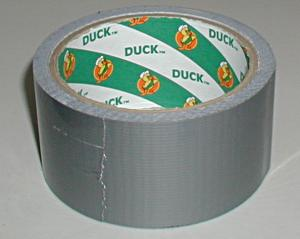
\includegraphics[scale=1.0,angle=-90]{pics/duck_tape.eps}
\end{center}
\vspace*{\fill}


\subsection{OS Installation}
Before installing, consider
\begin{itemize}
	\item installation process
		\begin{itemize}
			\item base installation
			\item installation of add-ons and third-party applications
			\item security implications
			\item able to be easily repeated
		\end{itemize}
	\item post-installation
		\begin{itemize}
			\item register information
			\item remove unneccessary software
			\item patch software
		\end{itemize}
\end{itemize}

\subsection{OS Installation}
Before installing, consider
\begin{itemize}
	\item installation process
		\begin{itemize}
			\item base installation
			\item installation of add-ons and third-party applications
			\item security implications
			\item able to be easily repeated
		\end{itemize}
	\item post-installation
		\begin{itemize}
			\item register information
			\item remove unneccessary software
			\item patch software
			\item disable services
		\end{itemize}
\end{itemize}

%\subsection{OS Installation}
%\vspace*{\fill}
%\begin{center}
%	\includegraphics[scale=0.8,angle=-90]{pics/inst-disklabel-partitions.eps}
%\end{center}
%\vspace*{\fill}
%
%\subsection{OS Installation}
%\vspace*{\fill}
%\begin{center}
%	\includegraphics[scale=0.55]{pics/disk.setup.eps}
%\end{center}
%\vspace*{\fill}
%
%\subsection{OS Installation}
%\vspace*{\fill}
%\begin{center}
%	\includegraphics[scale=0.8]{pics/install-ftp.eps}
%\end{center}
%\vspace*{\fill}
%
%\subsection{OS Installation}
%\vspace*{\fill}
%\begin{center}
%	\includegraphics[scale=0.8]{pics/nfssetup.eps}
%\end{center}
%\vspace*{\fill}
%
\subsection{OS Installation}
General steps:
\begin{itemize}
	\item boot from boot media (CD, network, ...)
\end{itemize}

\subsection{OS Installation}
General steps:
\begin{itemize}
	\item boot from boot media (CD, network, ...)
	\item identify root device
\end{itemize}

\subsection{OS Installation}
General steps:
\begin{itemize}
	\item boot from boot media (CD, network, ...)
	\item identify root device
	\item optionally identify additional devices
\end{itemize}

\subsection{OS Installation}
General steps:
\begin{itemize}
	\item boot from boot media (CD, network, ...)
	\item identify root device
	\item optionally identify additional devices
	\item create partition table / disklabel
\end{itemize}

\subsection{OS Installation}
General steps:
\begin{itemize}
	\item boot from boot media (CD, network, ...)
	\item identify root device
	\item optionally identify additional devices
	\item create partition table / disklabel
	\item create filesystem(s)
\end{itemize}

\subsection{OS Installation}
General steps:
\begin{itemize}
	\item boot from boot media (CD, network, ...)
	\item identify root device
	\item optionally identify additional devices
	\item create partition table / disklabel
	\item create filesystem(s)
	\item install MBR, bootblocks etc.
\end{itemize}

\subsection{OS Installation}
General steps:
\begin{itemize}
	\item boot from boot media (CD, network, ...)
	\item identify root device
	\item optionally identify additional devices
	\item create partition table / disklabel
	\item create filesystem(s)
	\item install MBR, bootblocks etc.
	\item install / copy / extract OS
\end{itemize}

\subsection{OS Installation}
General steps:
\begin{itemize}
	\item boot from boot media (CD, network, ...)
	\item identify root device
	\item optionally identify additional devices
	\item create partition table / disklabel
	\item create filesystem(s)
	\item install MBR, bootblocks etc.
	\item install / copy / extract OS
	\item optionally add application software
\end{itemize}

\subsection{OS Installation}
General steps:
\begin{itemize}
	\item boot from boot media (CD, network, ...)
	\item identify root device
	\item optionally identify additional devices
	\item create partition table / disklabel
	\item create filesystem(s)
	\item install MBR, bootblocks etc.
	\item install / copy / extract OS
	\item optionally add application software
	\item perform basic system configuration
\end{itemize}

\subsection{OS Installation}
General steps:
\begin{itemize}
	\item boot from boot media (CD, network, ...)
	\item identify root device
	\item optionally identify additional devices
	\item create partition table / disklabel
	\item create filesystem(s)
	\item install MBR, bootblocks etc.
	\item install / copy / extract OS
	\item optionally add application software
	\item perform basic system configuration
	\item reboot
\end{itemize}


\subsection{OS Installation}
``Any sufficiently advanced technology is indistinguishable from magic.''
\vspace*{\fill}
\begin{center}
	
\includegraphics[scale=0.5]{pics/magic_hat.eps}
\end{center}
\vspace*{\fill}


\newpage
\vspace*{\fill}
\begin{center}
	\Hugesize
		Software Installation Concepts \\ [1em]
	\hspace*{5mm}
	\blueline\\
	\hspace*{5mm}\\
		File System Hierarchy
\end{center}
\vspace*{\fill}

\subsection{File System Hierarchy}
Layout of filesystem {\em should} be standardized.  Some UNIX versions adhere
to these standards, some are strongly influenced by tradition.

\subsection{File System Hierarchy}
\vspace*{\fill}
\begin{center}
	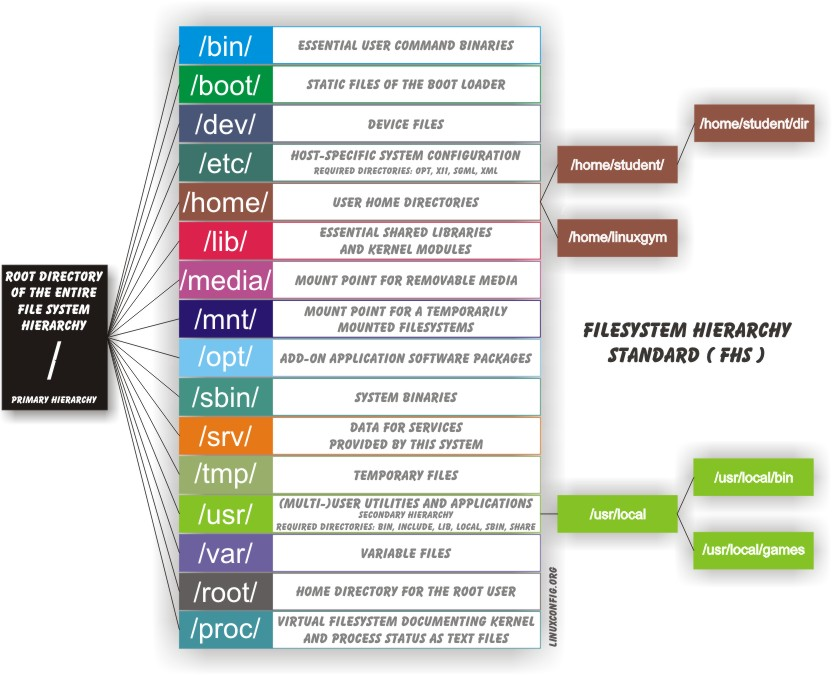
\includegraphics[scale=0.5,angle=-90]{pics/fhs.eps}
\end{center}
\vspace*{\fill}

\subsection{File System Hierarchy}
Layout of filesystem {\em should} be standardized.  Some UNIX versions adhere
to these standards, some are strongly influenced by tradition.
\\

Basic distinction between {\em shareable} and {\em unshareable} as well
as {\em static} and {\em variable} data.

\subsection{File System Hierarchy}
Layout of filesystem {\em should} be standardized.  Some UNIX versions adhere
to these standards, some are strongly influenced by tradition.
\\

Basic distinction between {\em shareable} and {\em unshareable} as well
as {\em static} and {\em variable} data.
\\

Shareable content:
\begin{itemize}
	\item essential components that remain the same across multiple hosts
	\item often possible to mount read-only
	\item may overlap with {\em local} data
\end{itemize}

\subsection{File System Hierarchy}
Layout of filesystem {\em should} be standardized.  Some UNIX versions adhere
to these standards, some are strongly influenced by tradition.
\\

Basic distinction between {\em shareable} and {\em unshareable} as well
as {\em static} and {\em variable} data.
\\

Shareable content:
\begin{itemize}
	\item essential components that remain the same across multiple hosts
	\item often possible to mount read-only
	\item may overlap with {\em local} data
\end{itemize}

Unshareable content:
\begin{itemize}
	\item data that needs to be individual to each host
	\item data that changes often
	\item may overlap with {\em local} data
\end{itemize}

\subsection{File System Hierarchy}
Examples:
\\

\begin{center}
\begin{tabular}{| l | l | l |}
	\hline
	& shareable content & unshareable content \\
	\hline
	static   & & \\
	         & & \\
	\hline
	variable & & \\
	         & & \\
	\hline
\end{tabular}
\end{center}


\subsection{File System Hierarchy}
Examples:
\\

\begin{center}
\begin{tabular}{| l | l | l |}
	\hline
	& shareable content & unshareable content \\
	\hline
	static   & \verb+/usr+ & \\
	         & \verb+/opt+ & \\
	\hline
	variable & & \\
	         & & \\
	\hline
\end{tabular}
\end{center}

\subsection{File System Hierarchy}
Examples:
\\

\begin{center}
\begin{tabular}{| l | l | l |}
	\hline
	& shareable content & unshareable content \\
	\hline
	static   & \verb+/usr+ & \verb+/etc+ \\
	         & \verb+/opt+ & \verb+/boot+ \\
	\hline
	variable & & \\
	         & & \\
	\hline
\end{tabular}
\end{center}

\subsection{File System Hierarchy}
Examples:
\\

\begin{center}
\begin{tabular}{| l | l | l |}
	\hline
	& shareable content & unshareable content \\
	\hline
	static   & \verb+/usr+ & \verb+/etc+ \\
	         & \verb+/opt+ & \verb+/boot+ \\
	\hline
	variable & \verb+/var/mail+ & \\
	         & \verb+/var/spool/news+ & \\
	\hline
\end{tabular}
\end{center}

\subsection{File System Hierarchy}
Examples:
\\

\begin{center}
\begin{tabular}{| l | l | l |}
	\hline
	& shareable content & unshareable content \\
	\hline
	static   & \verb+/usr+ & \verb+/etc+ \\
	         & \verb+/opt+ & \verb+/boot+ \\
	\hline
	variable & \verb+/var/mail+ & \verb+/var/run+ \\
	         & \verb+/var/spool/news+ & \verb+/var/lock+ \\
	\hline
\end{tabular}
\end{center}



\subsection{File System Hierarchy}
\begin{itemize}
	\item the root file system, or \verb+/+, needs to be adequate
		to boot, restore, recover, and/or repair the system.
	\item \verb+/usr+: often shareable, read-only data
	\item \verb+/usr/local+: truly {\em local} data; often mirrors
		\verb+/+ to a certain extent
	\item \verb+/var+: multi-purpose log, temporary, transient, and spool
		files; includes shareable and non-shareable data
\end{itemize}
See also: {\tt hier(7)}
\vspace{.5in}
Some Operating Systems may use other schemas.  Know thy enemy!

\newpage
\vspace*{\fill}
\begin{center}
    \Hugesize
        Hooray! \\ [1em]
    \hspace*{5mm}
    \blueline\\
    \hspace*{5mm}\\
        5 Minute Break
\end{center}
\vspace*{\fill}

\newpage
\vspace*{\fill}
\begin{center}
	\Hugesize
		Software Installation Concepts \\ [1em]
	\hspace*{5mm}
	\blueline\\
	\hspace*{5mm}\\
		System Software vs. Third Party Software
\end{center}
\vspace*{\fill}

\subsection{What's what?}
\subsection{What's what?}
\begin{center}
	\includegraphics[scale=0.9,angle=-90]{pics/kernel.eps}
\end{center}


\subsection{What's what?}
\begin{center}
	\includegraphics[scale=0.7]{pics/os.eps}
	\includegraphics[scale=0.7]{pics/beastie.eps}
\end{center}

\subsection{What's what?}
\begin{center}
	\includegraphics[scale=0.3,angle=-90]{pics/python.eps}
	\includegraphics[scale=0.3,angle=-90]{pics/logo_oracle.eps}
	\includegraphics[scale=0.8,angle=-90]{pics/apache.eps} \\
	\includegraphics[scale=0.3,angle=-90]{pics/mysql.eps}
	\includegraphics[scale=0.3,angle=-90]{pics/php-logo.eps}
\end{center}




\subsection{System Software vs. Third Party Software}
Consider:
\begin{itemize}
	\item OS upgrades vs. software upgrades
\end{itemize}

\subsection{System Software vs. Third Party Software}
Consider:
\begin{itemize}
	\item OS upgrades vs. software upgrades
	\item location of configuration files
\end{itemize}

\subsection{System Software vs. Third Party Software}
Consider:
\begin{itemize}
	\item OS upgrades vs. software upgrades
	\item location of configuration files
	\item duplicates or conflicting versions in the base system vs. the
		add-ons
\end{itemize}

\subsection{System Software vs. Third Party Software}
Consider:
\begin{itemize}
	\item OS upgrades vs. software upgrades
	\item location of configuration files
	\item duplicates or conflicting versions in the base system vs. the
		add-ons
	\item startup scripts, d{\ae}mons
\end{itemize}

\subsection{System Software vs. Third Party Software}
Consider:
\begin{itemize}
	\item OS upgrades vs. software upgrades
	\item location of configuration files
	\item duplicates or conflicting versions in the base system vs. the
		add-ons
	\item startup scripts, d{\ae}mons
	\item location of third party software
\end{itemize}

\subsection{System Software vs. Third Party Software}
Consider:
\begin{itemize}
	\item OS upgrades vs. software upgrades
	\item location of configuration files
	\item duplicates or conflicting versions in the base system vs. the
		add-ons
	\item startup scripts, d{\ae}mons
	\item location of third party software
	\item dependencies
\end{itemize}

\subsection{System Software vs. Third Party Software}
Consider:
\begin{itemize}
	\item OS upgrades vs. software upgrades
	\item location of configuration files
	\item duplicates or conflicting versions in the base system vs. the
		add-ons
	\item startup scripts, d{\ae}mons
	\item location of third party software
	\item dependencies
	\item installation by hand and/or installation using a package manager
\end{itemize}


\subsection{System Software vs. Third Party Software}
Consider:
\begin{itemize}
	\item OS upgrades vs. software upgrades
	\item location of configuration files
	\item duplicates or conflicting versions in the base system vs. the
		add-ons
	\item startup scripts, d{\ae}mons
	\item location of third party software
	\item dependencies
	\item installation by hand and/or installation using a package manager
	\item proprietary third party software
\end{itemize}

\subsection{More fun than...}
\vspace*{\fill}
\begin{center}
	\includegraphics[scale=0.7]{pics/bmonkey.eps}
\end{center}

\subsection{Binary vs. Source installation}
Benefits of binary installation:
\begin{itemize}
	\item packaged by "vendor" $\rightarrow$ support
\end{itemize}

\subsection{Binary vs. Source installation}
Benefits of binary installation:
\begin{itemize}
	\item packaged by "vendor" $\rightarrow$ support
	\item faster
\end{itemize}

\subsection{Binary vs. Source installation}
Benefits of binary installation:
\begin{itemize}
	\item packaged by "vendor" $\rightarrow$ support
	\item faster
	\item uses less space
\end{itemize}

\subsection{Binary vs. Source installation}
Benefits of binary installation:
\begin{itemize}
	\item packaged by "vendor" $\rightarrow$ support
	\item faster
	\item uses less space
	\item may be only possibility
\end{itemize}

\subsection{Binary vs. Source installation}
Benefits of binary installation:
\begin{itemize}
	\item packaged by "vendor" $\rightarrow$ support
	\item faster
	\item uses less space
	\item may be only possibility
	\item may be possible to deploy across large numbers of hosts
\end{itemize}

\subsection{Binary vs. Source installation}
Disadvantages of binary installation:
\begin{itemize}
	\item complex dependencies
\end{itemize}

\subsection{Binary vs. Source installation}
Disadvantages of binary installation:
\begin{itemize}
	\item complex dependencies
	\item installation procedure may be cumbersome
\end{itemize}

\subsection{Binary vs. Source installation}
Disadvantages of binary installation:
\begin{itemize}
	\item complex dependencies
	\item installation procedure may be cumbersome
	\item your OS may not be officially supported
\end{itemize}

\subsection{Binary vs. Source installation}
Disadvantages of binary installation:
\begin{itemize}
	\item complex dependencies
	\item installation procedure may be cumbersome
	\item your OS may not be officially supported
	\item installation scripts may be busted
\end{itemize}

\subsection{Binary vs. Source installation}
Disadvantages of binary installation:
\begin{itemize}
	\item complex dependencies
	\item installation procedure may be cumbersome
	\item your OS may not be officially supported
	\item installation scripts may be busted
	\item limited control over where files are installed
\end{itemize}

\subsection{Binary vs. Source installation}
Disadvantages of binary installation:
\begin{itemize}
	\item complex dependencies
	\item installation procedure may be cumbersome
	\item your OS may not be officially supported
	\item installation scripts may be busted
	\item limited control over where files are installed
	\item binaries not optimized for your systems
\end{itemize}

\subsection{Binary vs. Source installation}
Benefits of source installation:
\begin{itemize}
	\item full control over
		\begin{itemize}
			\item installation location
			\item compiler flags and optimization
			\item dependencies
		\end{itemize}
\end{itemize}

\subsection{Binary vs. Source installation}
Benefits of source installation:
\begin{itemize}
	\item full control over
		\begin{itemize}
			\item installation location
			\item compiler flags and optimization
			\item dependencies
		\end{itemize}
	\item make things work even if your OS is not officially supported
\end{itemize}

\subsection{Binary vs. Source installation}
Benefits of source installation:
\begin{itemize}
	\item full control over
		\begin{itemize}
			\item installation location
			\item compiler flags and optimization
			\item dependencies
		\end{itemize}
	\item make things work even if your OS is not officially supported
	\item ability to patch source (features, security etc.)
\end{itemize}

\subsection{Binary vs. Source installation}
Benefits of source installation:
\begin{itemize}
	\item full control over
		\begin{itemize}
			\item installation location
			\item compiler flags and optimization
			\item dependencies
		\end{itemize}
	\item make things work even if your OS is not officially supported
	\item ability to patch source (features, security etc.)
	\item able to integrate into your full OS image build
\end{itemize}

\subsection{Binary vs. Source installation}
Disadvantages of source installation:
\begin{itemize}
	\item complex dependencies
\end{itemize}

\subsection{Binary vs. Source installation}
Disadvantages of source installation:
\begin{itemize}
	\item complex dependencies
	\item may take time
\end{itemize}

\subsection{Binary vs. Source installation}
Disadvantages of source installation:
\begin{itemize}
	\item complex dependencies
	\item may take time
	\item requires more detailed knowledge
\end{itemize}

\subsection{Binary vs. Source installation}
Disadvantages of source installation:
\begin{itemize}
	\item complex dependencies
	\item may take time
	\item requires more detailed knowledge
	\item a lot of software is done poorly
\end{itemize}

\subsection{Binary vs. Source installation}
Disadvantages of source installation:
\begin{itemize}
	\item complex dependencies
	\item may take time
	\item requires more detailed knowledge
	\item a lot of software is done poorly
	\item not all software is available in source form
\end{itemize}

\subsection{More fun than...}
\vspace*{\fill}
\begin{center}
	\includegraphics[scale=0.7]{pics/headwall.eps}
\end{center}

\subsection{Build Automation}
\vspace*{\fill}
\begin{center}
	\includegraphics[scale=0.6,angle=-90]{pics/build-automation.eps}
\end{center}
\vspace*{\fill}


\newpage
\vspace*{\fill}
\begin{center}
	\Hugesize
		Software Installation Concepts \\ [1em]
	\hspace*{5mm}
	\blueline\\
	\hspace*{5mm}\\
		Package Management Systems
\end{center}
\vspace*{\fill}

\subsection{Why use a Package Management System?}
\vspace*{\fill}
\begin{center}
	\includegraphics[scale=0.4]{pics/cards.eps}
\end{center}
\vspace*{\fill}

\subsection{Why use a Package Management System?}
Sure, you {\em could} install everything by hand.  But ...

\subsection{Why use a Package Management System?}
Sure, you {\em could} install everything by hand.  But ...
\begin{itemize}
	\item thousands of applications and libraries are available
\end{itemize}

\subsection{Why use a Package Management System?}
Sure, you {\em could} install everything by hand.  But ...
\begin{itemize}
	\item thousands of applications and libraries are available
	\item binaries are not available for all platforms
\end{itemize}

\subsection{Why use a Package Management System?}
Sure, you {\em could} install everything by hand.  But ...
\begin{itemize}
	\item thousands of applications and libraries are available
	\item binaries are not available for all platforms
	\item compilation from source is not always trivial
\end{itemize}

\subsection{Why use a Package Management System?}
Sure, you {\em could} install everything by hand.  But ...
\begin{itemize}
	\item thousands of applications and libraries are available
	\item binaries are not available for all platforms
	\item compilation from source is not always trivial
		\begin{itemize}
			\item ``90\% of everything is crud''
		\end{itemize}
\end{itemize}

\subsection{Why use a Package Management System?}
Sure, you {\em could} install everything by hand.  But ...
\begin{itemize}
	\item thousands of applications and libraries are available
	\item binaries are not available for all platforms
	\item compilation from source is not always trivial
		\begin{itemize}
			\item ``90\% of everything is crud''
			\item platform and compiler issues may arise
		\end{itemize}
\end{itemize}

\subsection{Why use a Package Management System?}
Sure, you {\em could} install everything by hand.  But ...
\begin{itemize}
	\item thousands of applications and libraries are available
	\item binaries are not available for all platforms
	\item compilation from source is not always trivial
		\begin{itemize}
			\item ``90\% of everything is crud''
			\item platform and compiler issues may arise
			\item different ways of satisfying dependencies / optional
				features
		\end{itemize}
\end{itemize}

\subsection{Why use a Package Management System?}
Sure, you {\em could} install everything by hand.  But ...
\begin{itemize}
	\item thousands of applications and libraries are available
	\item binaries are not available for all platforms
	\item compilation from source is not always trivial
		\begin{itemize}
			\item ``90\% of everything is crud''
			\item platform and compiler issues may arise
			\item different ways of satisfying dependencies / optional
				features
		\end{itemize}
	\item how to maintain a database of installed applications?
\end{itemize}

\subsection{Why use a Package Management System?}
Sure, you {\em could} install everything by hand.  But ...
\begin{itemize}
	\item thousands of applications and libraries are available
	\item binaries are not available for all platforms
	\item compilation from source is not always trivial
		\begin{itemize}
			\item ``90\% of everything is crud''
			\item platform and compiler issues may arise
			\item different ways of satisfying dependencies / optional
				features
		\end{itemize}
	\item how to maintain a database of installed applications?
	\item dependencies among applications and libraries grow
		rather complex
\end{itemize}

\subsection{Complexity of Dependencies}
An example: Let's install some software to produce nice slides! \\

\vspace*{\fill}
\begin{center}
	\includegraphics[scale=1.0]{pics/xdvipresent.1.ps}
\end{center}

\subsection{Complexity of Dependencies}
An example: Let's install some software to produce nice slides! \\

\vspace*{\fill}
\begin{center}
	\includegraphics[scale=1.0]{pics/xdvipresent.2.ps}
\end{center}

\subsection{Complexity of Dependencies}
An example: Let's install some software to produce nice slides! \\

\vspace*{\fill}
\begin{center}
	\includegraphics[scale=0.8]{pics/xdvipresent.3.ps}
\end{center}

\subsection{Complexity of Dependencies}
An example: Let's install some software to produce nice slides (with
graphs)! \\

\vspace*{\fill}
\begin{center}
	\includegraphics[scale=0.65]{pics/xdvipresent.graphviz.ps}
\end{center}


\subsection{More fun than...}
\vspace*{\fill}
\begin{center}
	\includegraphics[scale=0.45]{pics/barrel_of_donkey.eps}
\end{center}

\subsection{Package Managment}
Important aspects of package managment:
\begin{itemize}
	\item available for virtually all OS (but different OS use
		different package managers)
\end{itemize}


\subsection{Package Managment}
Important aspects of package managment:
\begin{itemize}
	\item available for virtually all OS (but different OS use
		different package managers)
	\item may include building from source as well as (or) binary package
		managment
\end{itemize}

\subsection{Package Managment}
Important aspects of package managment:
\begin{itemize}
	\item available for virtually all OS (but different OS use
		different package managers)
	\item may include building from source as well as (or) binary package
		managment
	\item easily determine what is installed
\end{itemize}

\subsection{Package Managment}
Important aspects of package managment:
\begin{itemize}
	\item available for virtually all OS (but different OS use
		different package managers)
	\item may include building from source as well as (or) binary package
		managment
	\item easily determine what is installed
	\item keep track of {\em where} things are installed
\end{itemize}

\subsection{Package Managment}
Important aspects of package managment:
\begin{itemize}
	\item available for virtually all OS (but different OS use
		different package managers)
	\item may include building from source as well as (or) binary package
		managment
	\item easily determine what is installed
	\item keep track of {\em where} things are installed
	\item make {\em consistent} use of the package manager
\end{itemize}

\subsection{Package Managment}
Important aspects of package managment:
\begin{itemize}
	\item available for virtually all OS (but different OS use
		different package managers)
	\item may include building from source as well as (or) binary package
		managment
	\item easily determine what is installed
	\item keep track of {\em where} things are installed
	\item make {\em consistent} use of the package manager
	\item consider providing separate {\em depots} or {\em views} for
		different purposes
\end{itemize}

\subsection{Package Managment}
Important aspects of package managment:
\begin{itemize}
	\item available for virtually all OS (but different OS use
		different package managers)
	\item may include building from source as well as (or) binary package
		managment
	\item easily determine what is installed
	\item keep track of {\em where} things are installed
	\item make {\em consistent} use of the package manager
	\item consider providing separate {\em depots} or {\em views} for
		different purposes
	\item teach users to use the tools
\end{itemize}

\subsection{Package Managment}
Some popular package managment systems are:
\begin{itemize}
	\item Darwin and Mac OS X {\em fink} (and none)
	\item Debian packages (\verb+dpkg+, \verb+apt-get+)
	\item FreeBSD/OpenBSD {\em Ports}
	\item Gentoo Linux {\em portage}
	\item IRIX {\em tardist}
	\item NetBSD Packages Collection ({\em pkgsrc}) -- available for a
		wide range of platforms (*BSD, Linux, Solaris, Darwin, IRIX,
		HP-UX, AIX, ...)
	\item RedHat Package Manager (\verb+rpm+)
	\item Slackware Linux \verb+tgz+
	\item Solaris \verb+pkg+
	\item {\em Depot} and {\em GNU Stow}
\end{itemize}

\subsection{Managing Security Patches and Software Upgrades}
Always investigate {\em all} security issues relevant to your system!
\begin{itemize}
	\item consider escalation of low-level vulnerability to higher level
\end{itemize}

\subsection{Managing Security Patches and Software Upgrades}
Always investigate {\em all} security issues relevant to your system!
\begin{itemize}
	\item consider escalation of low-level vulnerability to higher level
	\item regularly check known resources
\end{itemize}

\subsection{Managing Security Patches and Software Upgrades}
Always investigate {\em all} security issues relevant to your system!
\begin{itemize}
	\item consider escalation of low-level vulnerability to higher level
	\item regularly check known resources
	\item use your vendor's security checking mechanism (if existent)
\end{itemize}

\subsection{Managing Security Patches and Software Upgrades}
Always investigate {\em all} security issues relevant to your system!
\begin{itemize}
	\item consider escalation of low-level vulnerability to higher level
	\item regularly check known resources
	\item use your vendor's security checking mechanism (if existent)
	\item consider impact of patches/upgrades
\end{itemize}

\subsection{Managing Security Patches and Software Upgrades}
Always investigate {\em all} security issues relevant to your system!
\begin{itemize}
	\item consider escalation of low-level vulnerability to higher level
	\item regularly check known resources
	\item use your vendor's security checking mechanism (if existent)
	\item consider impact of patches/upgrades
		\begin{itemize}
			\item dependencies
				\begin{itemize}
					\item shared libraries:  backwards compatibility, ABI
						changes?
					\item static libraries:  require update/rebuild
				\end{itemize}
		\end{itemize}
\end{itemize}

\subsection{Managing Security Patches and Software Upgrades}
Always investigate {\em all} security issues relevant to your system!
\begin{itemize}
	\item consider escalation of low-level vulnerability to higher level
	\item regularly check known resources
	\item use your vendor's security checking mechanism (if existent)
	\item consider impact of patches/upgrades
		\begin{itemize}
			\item dependencies
				\begin{itemize}
					\item shared libraries:  backwards compatibility, ABI
						changes?
					\item static libraries:  require update/rebuild
				\end{itemize}
			\item restart of binaries (reboot?)
		\end{itemize}
\end{itemize}

\subsection{Managing Security Patches and Software Upgrades}
Always investigate {\em all} security issues relevant to your system!
\begin{itemize}
	\item consider escalation of low-level vulnerability to higher level
	\item regularly check known resources
	\item use your vendor's security checking mechanism (if existent)
	\item consider impact of patches/upgrades
		\begin{itemize}
			\item dependencies
				\begin{itemize}
					\item shared libraries:  backwards compatibility, ABI
						changes?
					\item static libraries:  require update/rebuild
				\end{itemize}
			\item restart of binaries (reboot?)
			\item configuration file changes
		\end{itemize}
\end{itemize}

\subsection{Managing Security Patches and Software Upgrades}
Always investigate {\em all} security issues relevant to your system!
\begin{itemize}
	\item consider escalation of low-level vulnerability to higher level
	\item regularly check known resources
	\item use your vendor's security checking mechanism (if existent)
	\item consider impact of patches/upgrades
		\begin{itemize}
			\item dependencies
				\begin{itemize}
					\item shared libraries:  backwards compatibility, ABI
						changes?
					\item static libraries:  require update/rebuild
				\end{itemize}
			\item restart of binaries (reboot?)
			\item configuration file changes
			\item user interface
		\end{itemize}
\end{itemize}

\subsection{Managing Security Patches and Software Upgrades}
Always investigate {\em all} security issues relevant to your system!
\begin{itemize}
	\item consider escalation of low-level vulnerability to higher level
	\item regularly check known resources
	\item use your vendor's security checking mechanism (if existent)
	\item consider impact of patches/upgrades
		\begin{itemize}
			\item dependencies
				\begin{itemize}
					\item shared libraries:  backwards compatibility, ABI
						changes?
					\item static libraries:  require update/rebuild
				\end{itemize}
			\item restart of binaries (reboot?)
			\item configuration file changes
			\item user interface
			\item conflict with system requirements
		\end{itemize}
\end{itemize}

\subsection{Managing Security Patches and Software Upgrades}
Always investigate {\em all} security issues relevant to your system!
\begin{itemize}
	\item consider escalation of low-level vulnerability to higher level
	\item regularly check known resources
	\item use your vendor's security checking mechanism (if existent)
	\item consider impact of patches/upgrades
		\begin{itemize}
			\item dependencies
				\begin{itemize}
					\item shared libraries:  backwards compatibility, ABI
						changes?
					\item static libraries:  require update/rebuild
				\end{itemize}
			\item restart of binaries (reboot?)
			\item configuration file changes
			\item user interface
			\item conflict with system requirements
		\end{itemize}
	\item verify your vendor's patches integrity
\end{itemize}

\subsection{Managing Security Patches and Software Upgrades}
Always investigate {\em all} security issues relevant to your system!
\begin{itemize}
	\item consider escalation of low-level vulnerability to higher level
	\item regularly check known resources
	\item use your vendor's security checking mechanism (if existent)
	\item consider impact of patches/upgrades
		\begin{itemize}
			\item dependencies
				\begin{itemize}
					\item shared libraries:  backwards compatibility, ABI
						changes?
					\item static libraries:  require update/rebuild
				\end{itemize}
			\item restart of binaries (reboot?)
			\item configuration file changes
			\item user interface
			\item conflict with system requirements
		\end{itemize}
	\item verify your vendor's patches integrity
	\item if no patches are available, {\em make your own}
\end{itemize}

\subsection{HW \#2}
Package Management on different OS
\\

Detailed homework assignment posted at
\verb+http://www.cs.stevens.edu/~jschauma/615/s12-hw2.html+


\subsection{Links}
\begin{itemize}
	\item \verb+http://www.pathname.com/fhs/+
	\item hier(7)
	\item your package managers' manual pages
		\begin{itemize}
			\item pkg\_info(1)
			\item pkginfo(1), pkgadd(1M)
			\item rpm(1)
			\item ...
		\end{itemize}
	\item \verb+http://www.pkgsrc.org/+
\end{itemize}

\end{document}
